\documentclass[a4paper,12pt]{article}
\usepackage[utf8]{inputenc}
\usepackage{geometry}
\usepackage{graphicx}
\usepackage{listings}
\usepackage{xcolor}
\usepackage{tikz}
\usepackage{float} 
\usetikzlibrary{shapes, arrows, positioning, fit, calc}

% Config
\definecolor{codegreen}{rgb}{0,0.6,0}
\definecolor{codegray}{rgb}{0.5,0.5,0.5}
\definecolor{backcolour}{rgb}{0.95,0.95,0.92}

\lstdefinestyle{mystyle}{
    backgroundcolor=\color{backcolour},   
    commentstyle=\color{codegreen},
    basicstyle=\ttfamily\footnotesize,
    breakatwhitespace=false,         
    breaklines=true,                 
    captionpos=b,                    
    keepspaces=true,                 
    numbers=left,                    
    numbersep=5pt,                  
    showspaces=false,                
    showtabs=false,                  
    tabsize=2,
    frame=single
}
\lstset{style=mystyle}

\title{Practical Work 5: The Longest Path with MapReduce}
\author{Le Quy Ton \\ 23BI14425}
\date{\today}

\begin{document}

\maketitle

\section{Introduction}
This practical work focuses on finding the longest file path(s) within a distributed file system simulation using the MapReduce paradigm.The goal is to process a set of file paths (simulating output from \texttt{find /}) and efficiently identify the path string with the maximum character count.

\section{Implementation Choice}
Similar to the previous Word Count exercise, we utilize the \emph{Python Streaming} approach combined with Linux utilities, adhering to the "Invent yourself" requirement.

\begin{itemize}
    \item \textbf{Mapper:} Written in Python. It calculates the length of each path string.
    \item \textbf{Shuffle/Sort:} Utilizes the Linux \texttt{sort -n -r} command. The flags \texttt{-n} (numeric) and \texttt{-r} (reverse) are crucial to place the longest paths at the top of the stream.
    \item \textbf{Reducer:} Written in Python. It reads the sorted stream and outputs the top element(s).
\end{itemize}

\section{System Design and Operation}

\subsection{Mapper Logic}
The Mapper reads file paths line by line. For each path, it computes the string length and emits a key-value pair: $<Length, Path>$.
Example: Input \texttt{/usr/bin} $\rightarrow$ Output \texttt{8\textbackslash t/usr/bin}.

\subsection{Reducer Logic}
The Reducer receives input sorted by Length in descending order. It captures the length of the very first record (the maximum length). It then prints every path matching this length and terminates immediately upon encountering a shorter path, ensuring efficiency.

\subsection{Process Visualization}
Figure \ref{fig:longestpath} illustrates the data flow for finding the longest path.

\begin{figure}[H]
    \centering
    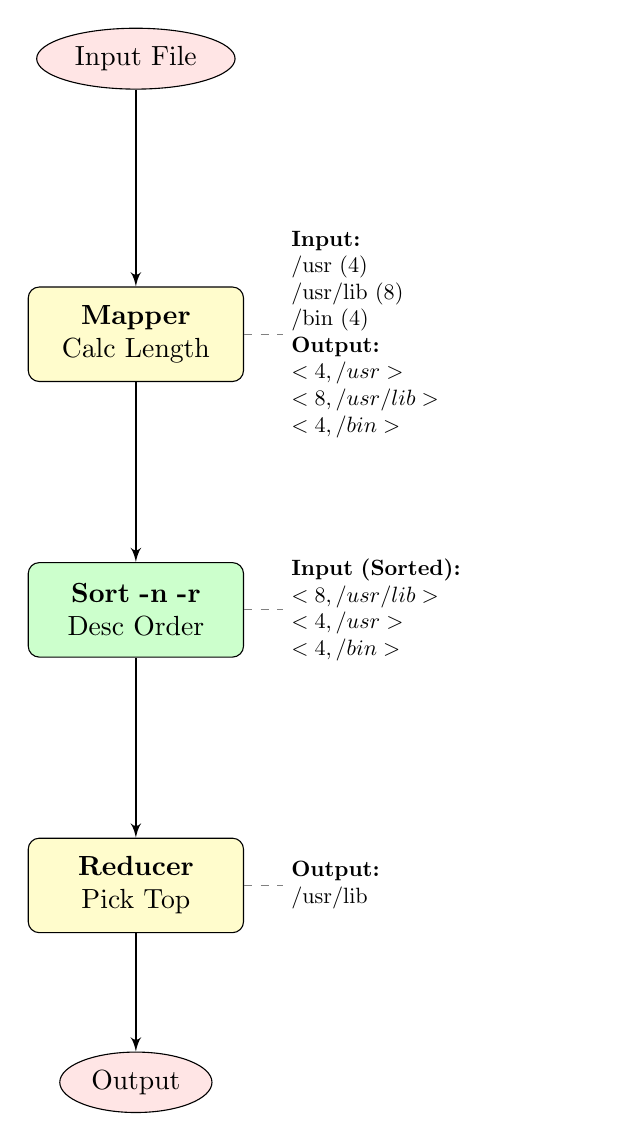
\begin{tikzpicture}[node distance=3.5cm, auto,
        block/.style={rectangle, draw, fill=blue!10, text width=2.5cm, align=center, rounded corners, minimum height=1.2cm},
        cloud/.style={draw, ellipse, fill=red!10, node distance=3.5cm, minimum height=2em},
        line/.style={draw, -latex', thick}]

        % Nodes
        \node [cloud] (input) {Input File};
        \node [block, below of=input, fill=yellow!20] (map) {\textbf{Mapper}\\ Calc Length};
        \node [block, below of=map, fill=green!20] (shuffle) {\textbf{Sort -n -r}\\Desc Order};
        \node [block, below of=shuffle, fill=yellow!20] (reduce) {\textbf{Reducer}\\Pick Top};
        \node [cloud, below of=reduce, node distance=2.5cm] (output) {Output};

        % Data annotations
        \node [right=0.5cm of map, text width=5cm, scale=0.8, align=left] (mapdata) {
            \textbf{Input:} \\
            /usr (4) \\
            /usr/lib (8) \\
            /bin (4) \\
            \textbf{Output:} \\
            $<4, /usr>$ \\
            $<8, /usr/lib>$ \\
            $<4, /bin>$
        };
        
        \node [right=0.5cm of shuffle, text width=5cm, scale=0.8, align=left] (shuffledata) {
            \textbf{Input (Sorted):}\\
            $<8, /usr/lib>$ \\
            $<4, /usr>$ \\
            $<4, /bin>$
        };

        \node [right=0.5cm of reduce, text width=5cm, scale=0.8, align=left] (reducedata) {
            \textbf{Output:}\\
            /usr/lib
        };

        % Paths
        \path [line] (input) -- (map);
        \path [line] (map) -- (shuffle);
        \path [line] (shuffle) -- (reduce);
        \path [line] (reduce) -- (output);
        
        % Drawing lines to annotations
        \draw [dashed, gray] (map) -- (mapdata);
        \draw [dashed, gray] (shuffle) -- (shuffledata);
        \draw [dashed, gray] (reduce) -- (reducedata);

    \end{tikzpicture}
    \caption{Workflow of the Longest Path MapReduce}
    \label{fig:longestpath}
\end{figure}

\section{Execution and Results}
We verified the implementation by creating a sample input file containing paths of various lengths. The pipeline was executed using the standard Linux command line. Figure \ref{fig:execution} shows the terminal output. The system correctly identified \texttt{/home/user/documents/report.pdf} as the longest path from the provided input list.

\begin{figure}[H]
    \centering
    
\includegraphics[width=1.0\linewidth]{image1.png}
    \caption{Successful execution of Longest Path MapReduce}
    \label{fig:execution}
\end{figure}

\section{Code Implementation}

\subsection{Mapper (mapper.py)}
\begin{lstlisting}[language=Python]
import sys
for line in sys.stdin:
    path = line.strip()
    if path:
        # Emit length first for sorting
        print(f"{len(path)}\t{path}")
\end{lstlisting}

\subsection{Reducer (reducer.py)}
\begin{lstlisting}[language=Python]
import sys
max_len = -1
for line in sys.stdin:
    try:
        len_str, path = line.strip().split('\t', 1)
        length = int(len_str)
        
        if max_len == -1: max_len = length
        
        if length == max_len:
            print(path) # Found a longest path
        elif length < max_len:
            break # Stop processing since list is sorted desc
    except ValueError: continue
\end{lstlisting}

\section{Conclusion}
We successfully implemented the Longest Path problem using a MapReduce pipeline. The key difference from Word Count is the sorting strategy: by emitting the length as the key and sorting numerically in reverse (\texttt{sort -n -r}), the Reducer only needs to process the first few lines to find the global maximum. This demonstrates the flexibility of the MapReduce model for different types of aggregation tasks.

\end{document}
